\documentclass[fleqn,10pt]{wlscirep}
\usepackage[utf8]{inputenc}
\usepackage[T1]{fontenc}
\usepackage{lineno}
\linenumbers

\title{A Comprehensive Dataset of U.S. Laws }

\author[$\dag$]{Brian Libgober}
\affil[$\dag$]{Northwestern University, Department of Political Science and School of Law, Evanston, IL, 60202, USA. brian.libgober@northwestern.edu}


\begin{abstract}
Lists of US laws figure importantly in many research projects in political science, law, sociology, economics, and other disciplines. Yet despite their prominence and frequent use, there is no authoritative and complete dataset of all US laws. In part, this is because US laws have been enacted over hundreds of years, resulting in a complicated patchwork published in numerous and inconsistent formats. As a simplification, many scholars have relied upon more selective lists of \textit{major} legislative enactments, although the selection criteria for these narrower lists make their use questionable in many cases. Here, we describe our efforts to create a complete database of US laws and their revision histories by combining data from HEINOnline and Congress.gov.
\end{abstract}

\begin{document}

\flushbottom
\maketitle
%  Click the title above to edit the author information and abstract

\thispagestyle{empty}

\section*{Background \& Summary}

%(700 words maximum) An overview of the study design, the assay(s) performed, and the created data, including any background information needed to put this study in the context of previous work and the literature. The section should also briefly outline the broader goals that motivated the creation of this dataset and the potential reuse value. We also encourage authors to include a figure that provides a schematic overview of the study and assay(s) design. The Background \& Summary should not include subheadings. This section and the other main body sections of the manuscript should include citations to the literature as needed. 

In the US federal system, laws in the sense of ordinary usage can originate from many sources, including Courts, the President, agencies, and so forth. Yet when scholars speak more formally about the set of "US laws," they typically intend to refer to the set of authoritative documents enacted by the two chambers of the US Congress by following the legislative process. When Congress acts legislatively, it may do so by issuing a variety of documents that go by different names, have different formal features, and follow different processes. At present writing, the set of allowable actions include bills, joint resolutions, concurrent resolutions, and simple resolutions. Of these, only bills and joint resolutions have the general and binding character that one typically associates with laws. And even then, there are exceptions within these categories. ``Private bills" granting relief in one-off cases\footnote{For example, last year Congress enacted a private law allowing Alaska-woman Rebecca Trimble to obtain permanent resident status, despite the fact the paperwork her adoptive parents had used to bring her to the United States from Mexico had been defective.} are typically not what scholars have in mind when one refers to ``laws'', nor are joint resolutions approving constitutional amendments which are not ratified by the states (e.g. the Equal Rights Amendment) really laws. That said, the set of enacted bills and joint resolutions is a relatively precise definition of what scholars \textit{should} mean when they talk about the set of US federal laws.

Studies of lawmaking in US political science are not new. Indeed, a very important debate in political science over the past several decades has to do with whether unified government, where the President and Congress are controlled by the same party, is better or worse for legislative productivity than divided government, where these organs are not exclusively in controlled by the same political party. This debate was initiated by Mayhew (1991) \nocite{Mayhew1991}, who published a list of ``major'' legislative enactments identified by the set of laws that were mentioned in the editorial page of the New York Times and other prominent newspapers. This list of major enactments has been updated annually since its original publication in 1991 and is, at present writing, current from 1947 through 2022. Of course, the coverage of major legislative enactments is obviously limited as a database of all federal laws, both because it does not cover laws that fail to draw the attention of editorial pages, nor does it cover laws enacted during the New Deal or earlier. 

Addressing these weaknesses has been the subject of at least two other major research projects. The Policy Agendas Project is a long-standing collaborative research effort aimed at building multiple datasets for tracking and comparing which issues manage to attract the attention of government across. It covers many national and subnatnional systems, including hte United States federal government. In particular, their database of bills covers "more than 400,000 bills introduced by the US Congress." Importantly, they also have coded each bill according to the subject-matter coding system of the larger Policy Agenda Project. Their focus on covering the subject matter of lawmaking is an important undertaking, although arduous, and it is unsurprising given the difficulties of this undertaking that they have only managed to cover the period 1947-2022. The second project with relevant and similar prior data collection is due to Ansolabehere, Palmer, and Schneer.\cite{ansolabehere_palmer_schneer_2016,ansolabehere2018divided} Their data collection, which was conducted under the auspices of an undergraduate course at Harvard called ``"What Has Congress Done," crowd-sourced the task of identifying significant legislation to students, each of whom was responsible for producing a list of significant legislation enacted under each of 22 potentially assigned decades. The researchers provided a list of secondary sources, as well as guidance and quality control efforts. Similar to Mayhew, their criteria for inclusion were (a) was the law considered significant at the time of enactment, and (b) does the law seem significant in historical perspective. Because of their differing methods, the two sources do not completely overlap in the 1947-2022 period. Although the temporal coverage for the Ansolabehere, Palmer, and Schneer dataset is very comprehensive, it contains a small percentage of all laws enacted by the US Congress.

% A few OTHER PAPERS
% Clinton and Lapinski (2006)
% Stathis (2014)
% Howell, William, Scott Adler, Charles Cameron, and Charles Riemann (2000) “Divided government
and the legislative productivity of Congress, %1945–94.” Legislative Studies Quarterly 25 (2): 285–
%312

There are several reasons why it is desirable to have a more complete dataset of US lawmaking than has previously existed. In particular, minor legislation is usually major to somebody, otherwise they would not go through the trouble of passing it. While focusing on the big pieces of legislation is perhaps appropriate for thinking about how party control effects the ability of collective government to solve the big problems, a more granular perspective is really necessary to think about how special interests may whittle away the gains made by broad coalitions through smaller pieces of legislation, or perhaps how policy fails to make the necessary incremental adjustments to keep with the times. There is notable inconsistency in what laws are included as significant using all these methods. The lack of a unified and complete dataset also frustrates progress of the discipline, as these authors do not necessarily use the same system to refer to particular laws, making US law datasets used by social scientist less inter-operable than they should be. 

Our project seeks to build a comprehensive and easily updated list of US laws and their revision histories based on publicly available sources. The two key sources we leverage are the Statutes at Large, for laws existing before 2012, and Congress.gov, for more recent laws. The Congress.gov component is downloadable by webscraping and is relatively uncomplicated.  The more challenging part of the project involves cataloguing the older set of laws contained within the Statutes at Large. Surprisingly, the US government does not make electronic copies of the Statutes at Large available prior to 1951,\footnote{https://www.govinfo.gov/app/collection/statute/2016}, despite the fact that there were 64 earlier volumes containing laws that in many cases have not been amended. Despite the surprising limited availability of these foundational documents, a database widely used by legal scholars, HeinOnline, has digitized all these books in their entirety and provided meta data on their table of contents. Laws are identified in the statutes of laws in various and not perfectly ways across the decades. For this reason, we supply a more consistent set of identifiers that, going forward, allows laws to be easily matched by researchers. We describe these identifiers in more detail in the usage section below. Additionally, we include a set of text data that corresponds to these laws, although particularly for earlier laws these are collected via OCR. 

\section*{Methods}

We rely on two primary sources for our comprehensive database of US laws: the U.S. Statutes at Large, as disseminated via HeinOnline, and Congress.gov. 

For our data collection based on HeinOnline, we began by scraping the table of contents of each volume of the statues at large, excepting volumes 6-8 which contain a collection of early treaties and private laws. Examination of these tables reveals that laws are identified using various citation systems depending on era. In particular,

\begin{itemize}
\item The currently practiced identification system begins on Jan 7, 1959 with the 86th Congress. In this system, laws are identified by the number of the Congress and the law number within Congress. An example is ``Public Law 105-89, An Act: to promote the adoption of children in foster care.'' 
\item Initially, laws were identified by a different system. From the 1st through the 56th Congress, which concluded March 3, 1901, laws were identified in the Statutes at Large by chapter as well as Congress and session (e.g. ``Chapter 15, 56 Congress, Session 1, An Act: Relating to Cuban vessels.") 
\item For the 57th through 85th congress, the Statutes at Large inconsistently use both systems, with the important caveat that chapters and public laws are sometimes recycled over the two sessions of a particular Congress.\footnote{Or worse, the same session. Indeed, PL 65-246 refers to both a law ``Providing for the transportation from the District of Columbia of governmental employees whose services no longer are required." and also a law intended ``To authorize the sale of certain lands to school district numbered twenty-eight, of Missoula County, Montana."} Careful attention to chapters, public laws, and sessions does disambiguate all laws, however these details are very particular and subtle. 
\end{itemize}

Following these citation practices, we used a rule-based parser to extract key pieces of information to identify the law. Technical validation efforts revealed that there were occasional errors of transcription in our source data, for example mis-identification of chapters associated with laws or including page numbers that were not correct. Those errors that were found in the source data we corrected to conform with the text image captured on the HeinOnline site. 


% The Methods should include detailed text describing any steps or procedures used in producing the data, including full descriptions of the experimental design, data acquisition assays, and any computational processing (e.g. normalization, image feature extraction). See the detailed section in our submission guidelines for advice on writing a transparent and reproducible methods section. Related methods should be grouped under corresponding subheadings where possible, and methods should be described in enough detail to allow other researchers to interpret and repeat, if required, the full study. Specific data outputs should be explicitly referenced via data citation (see Data Records and Citing Data, below).

% Authors should cite previous descriptions of the methods under use, but ideally the method descriptions should be complete enough for others to understand and reproduce the methods and processing steps without referring to associated publications. There is no limit to the length of the Methods section. Subheadings should not be numbered.

% \subsection*{Subsection}

% Example text under a subsection. Bulleted lists may be used where appropriate, e.g.

% \begin{itemize}
% \item First item
% \item Second item
% \end{itemize}

% \subsubsection*{Third-level section}
 
% Topical subheadings are allowed.

\section*{Data Records}

% The Data Records section should be used to explain each data record associated with this work, including the repository where this information is stored, and to provide an overview of the data files and their formats. Each external data record should be cited numerically in the text of this section, for example \cite{Hao:gidmaps:2014}, and included in the main reference list as described below. A data citation should also be placed in the subsection of the Methods containing the data-collection or analytical procedure(s) used to derive the corresponding record. Providing a direct link to the dataset may also be helpful to readers (\hyperlink{https://doi.org/10.6084/m9.figshare.853801}{https://doi.org/10.6084/m9.figshare.853801}).

% Tables should be used to support the data records, and should clearly indicate the samples and subjects (study inputs), their provenance, and the experimental manipulations performed on each (please see 'Tables' below). They should also specify the data output resulting from each data-collection or analytical step, should these form part of the archived record.

\section*{Technical Validation}

% This section presents any experiments or analyses that are needed to support the technical quality of the dataset. This section may be supported by figures and tables, as needed. This is a required section; authors must present information justifying the reliability of their data.

We offer two primary approaches to support the technical validation of our dataset. The first is to compare the total counts of laws by Congress against previously published totals while the second validation exercise is to show that all of the laws described in five distinct sources of major laws are, indeed, present in our dataset.

The reference counts for total laws that we rely on comes from Appendix F reported in Galloway and Wise's History of the House of Representatives, and also previously used for validation and analysis by Ansolabhere, Palmer, and Schneer.\cite{ansolabehere_palmer_schneer_2016} Our definition of law is slightly more capacious than theirs, in the sense that we also consider "Joint Resolutions" laws, and the authors admit their own counts combine acts and resolutions (the latter of which are not, in our view, best understood as laws) from the 77th Congress and after. Figure \ref{fig:totals} compares the counts for this key subset of our data. Note that the total deviation in counts is X. An undergraduate research assistant further investigated the difference in counts of laws in Congress A and B. In both cases, the number of laws that the research assistant counted in that Congress was the same as the number we provided. 

A second 
\

\section*{Usage Notes}  \label{sec:usage}

% The Usage Notes should contain brief instructions to assist other researchers with reuse of the data. This may include discussion of software packages that are suitable for analysing the assay data files, suggested downstream processing steps (e.g. normalization, etc.), or tips for integrating or comparing the data records with other datasets. Authors are encouraged to provide code, programs or data-processing workflows if they may help others understand or use the data. Please see our code availability policy for advice on supplying custom code alongside Data Descriptor manuscripts.

% For studies involving privacy or safety controls on public access to the data, this section should describe in detail these controls, including how authors can apply to access the data, what criteria will be used to determine who may access the data, and any limitations on data use. 

\section*{Code availability}

% For all studies using custom code in the generation or processing of datasets, a statement must be included under the heading "Code availability", indicating whether and how the code can be accessed, including any restrictions to access. This section should also include information on the versions of any software used, if relevant, and any specific variables or parameters used to generate, test, or process the current dataset. 

\bibliography{biblio}

% \noindent LaTeX formats citations and references automatically using the bibliography records in your .bib file, which you can edit via the project menu. Use the cite command for an inline citation, e.g. \cite{Kaufman2020, Figueredo:2009dg, Babichev2002, behringer2014manipulating}. For data citations of datasets uploaded to e.g. \emph{figshare}, please use the \verb|howpublished| option in the bib entry to specify the platform and the link, as in the \verb|Hao:gidmaps:2014| example in the sample bibliography file. For journal articles, DOIs should be included for works in press that do not yet have volume or page numbers. For other journal articles, DOIs should be included uniformly for all articles or not at all. We recommend that you encode all DOIs in your bibtex database as full URLs, e.g. https://doi.org/10.1007/s12110-009-9068-2.

\section*{Acknowledgements} (not compulsory)

% Acknowledgements should be brief, and should not include thanks to anonymous referees and editors, or effusive comments. Grant or contribution numbers may be acknowledged.

\section*{Author contributions statement}

% Must include all authors, identified by initials, for example:
% A.A. conceived the experiment(s), A.A. and B.A. conducted the experiment(s), C.A. and D.A. analysed the results. All authors reviewed the manuscript. 

\section*{Competing interests} (mandatory statement)

% The corresponding author is responsible for providing a \href{https://www.nature.com/sdata/policies/editorial-and-publishing-policies#competing}{competing interests statement} on behalf of all authors of the paper. This statement must be included in the submitted article file.

\section*{Figures \& Tables}

% Figures, tables, and their legends, should be included at the end of the document. Figures and tables can be referenced in \LaTeX{} using the ref command, e.g. Figure \ref{fig:stream} and Table \ref{tab:example}. 

% Authors are encouraged to provide one or more tables that provide basic information on the main ‘inputs’ to the study (e.g. samples, participants, or information sources) and the main data outputs of the study. Tables in the manuscript should generally not be used to present primary data (i.e. measurements). Tables containing primary data should be submitted to an appropriate data repository.

% Tables may be provided within the \LaTeX{} document or as separate files (tab-delimited text or Excel files). Legends, where needed, should be included here. Generally, a Data Descriptor should have fewer than ten Tables, but more may be allowed when needed. Tables may be of any size, but only Tables which fit onto a single printed page will be included in the PDF version of the article (up to a maximum of three). 

% Due to typesetting constraints, tables that do not fit onto a single A4 page cannot be included in the PDF version of the article and will be made available in the online version only. Any such tables must be labelled in the text as ‘Online-only’ tables and numbered separately from the main table list e.g. ‘Table 1, Table 2, Online-only Table 1’ etc.

% \begin{figure}[ht]
% \centering
% 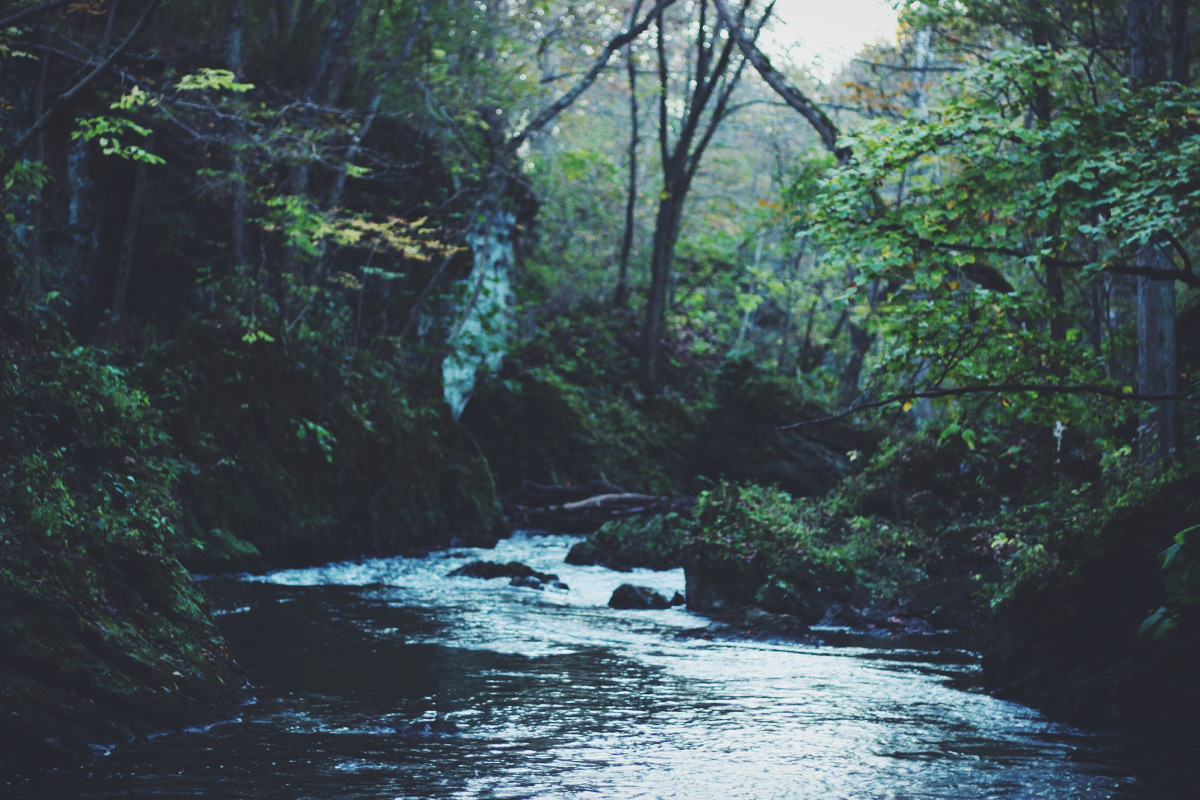
\includegraphics[width=\linewidth]{./assets/stream}
% \caption{Legend (350 words max). Example legend text.}
% \label{fig:stream}
% \end{figure}

% \begin{table}[ht]
% \centering
% \begin{tabular}{|l|l|l|}
% \hline
% Condition & n & p \\
% \hline
% A & 5 & 0.1 \\
% \hline
% B & 10 & 0.01 \\
% \hline
% \end{tabular}
% \caption{\label{tab:example}Legend (350 words max). Example legend text.}
% \end{table}

\end{document}